Aplikace je prostředníkem mezi RÚIAN VFR a~cílovou databází.
Hlavním úkolem je stažení dat z~RÚIAN VFR, jejich přečtení, zpracování a~následné uložení do cílové databáze.
Aplikace bude psána v~jazyce Java. Bude třeba zajistit funkce pro zpracování a~uložení dat.
Dále bude třeba zajisti, aby se aplikace věděla, co bude dělat a~jak se chovat.
Pro toto bude třeba vytvořit konfigurační soubor, který bude obsahovat nastavení aplikace.
Na obrázku \ref{fig:architektura} je znázorněna architektura aplikace.
Zelené šipky popisují směr toku dat.
Červené šipky popisují ovládací signály.

\begin{figure}[!h]
    \centering
    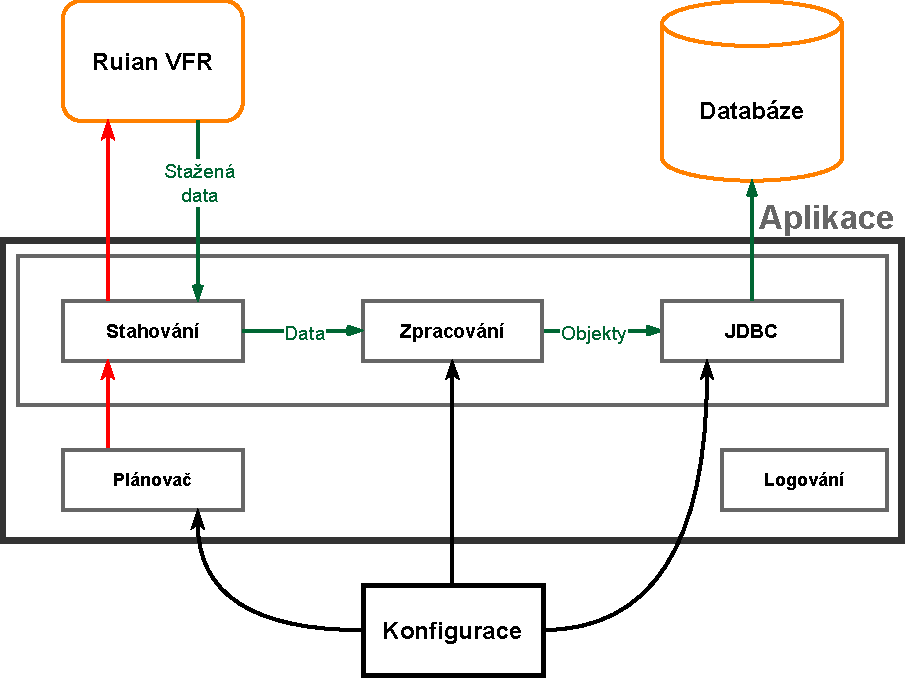
\includegraphics[width=0.8\textwidth]{figures/Aplikace_Scheme.pdf}
    \caption{Architektura aplikace}
    \label{fig:architektura}
\end{figure}

\newpage

\section{Stahování dat}
Stahování dat bude zajištěno pomocí knihovny \textit{Apache HttpClient}, která je
součástí balíčku \textit{Apache HttpComponents}.
Tato knihovna umožňuje snadné a~efektivní stahování dat z~webových stránek a~API.
V~rámci této aplikace bude použita k~stahování dat z~RÚIAN VFR.
Data budou stažena jako ZIP soubor, který bude následně rozbalen a~zpracován.
Soubory budou uloženy do dočasného adresáře, který bude po zpracování smazán z~důvodu úspory volného místa.

\section{Zpracování dat}
Zpracování dat se bude skládat z~několika částí.
Přečtení a~mapování dat do objektů, které budou následně uloženy do databáze.
Pro čtení dat bude třeba parser XML souborů, který přečte data a~převede je do objektů.
Vzhledem k~velikosti dat bude třeba zajistit efektivní zpracování, aby nedocházelo
k~přetížení paměti a~CPU.
Pro čtení je možné využít knihovnu \textit{Jackson} nebo \textit{StAX}.

\begin{enumerate}
    \item \textbf{Jackson} -- knihovna pro zpracování JSON a~XML dat. Umožňuje snadné mapování
    objektů na JSON a~XML a~naopak. Je velmi rychlá a~efektivní, ale může být složitější na použití.
    \item \textbf{StAX} -- knihovna pro zpracování XML dat. Umožňuje
    čtení a~zápis XML dat pomocí událostí. Je velmi rychlá a~efektivní, ale může být
    složitější na použití.
\end{enumerate}

Vybrán byl parser \textbf{StAX}, z~důvodů snadného použití a~rychlosti.
Také nepotřebuje mít načtený celý soubor do paměti, ale čte jako proud.

Následně bude třeba vytvořit objekty pro mapování dat do objektů.
Tyto objekty budou mít stejnou strukturu jako data z~RÚIAN VFR.
Pro mapování bude využita knihovna \textit{JPA} (Java Persistence API), která umožňuje snadné
mapování objektů na databázové tabulky a~naopak.
Pro tuto technologii je třeba vytvořit databázové entity, které budou mít stejnou strukturu jako
v~databázi. Dále bude třeba vytvořit repositáře pro práci s~databází (CRUD operace).
A nakonec bude třeba vytvořit služby, které budou sloužit pro práci s~repositáři a~pro zpracování dat.

Před uložením do databáze bude třeba provést validaci dat, aby nedocházelo k~chybám při
ukládání. Je třeba zajistit, aby se zabránilo ukládání dat, která jsou neplatná nebo nekompletní.
Možné chyby při validaci dat:
\begin{itemize}
    \item Chybějící primární klíče.
    \item Nevalidní cizí klíče.
\end{itemize}

\section{Komunikace s~databází}
\label{sec:komunikaceDB}
Pro ukládání dat je třeba se nejprve připojit k~databázi.
Pro připojení k~databázi bude použita knihovna \textit{JDBC} (Java Database Connectivity), která
umožňuje připojení k~různým databázím pomocí standardního API.
Jednotlivé databáze budou vyžadovat různé \textit{JDBC} ovladače, které umožňují připojení k~vybraným databázím.

Pro připojení k~databázi bude třeba vytvořit konfigurační soubor, který bude obsahovat
informace o~připojení k~databázi.

\section{Formát konfiguračního souboru}
Je třeba zajistit, aby aplikace byla schopna načíst konfigurační soubor a~podle něj se správně nakonfigurovat.
Je tedy nutné zvolit vhodný formát tohoto souboru.
Existuje několik možností, z~nichž je třeba vybrat tu nejvhodnější:

\begin{itemize}
    \item \textbf{XML (XSD)} -- Extensible Markup Language,
    \item \textbf{JSON} -- JavaScript Object Notation,
    \item \textbf{YAML} -- YAML Ain't Markup Language,
    \item \textbf{INI} -- Initialization File,
\end{itemize}

\subsection{XML}
XML je značkovací jazyk, na rozdíl od JSON a~YAML.
Jedná se o~textový formát, který však není tak snadno čitelný pro člověka jako JSON nebo YAML.
Podporuje víceúrovňovou strukturu a~komentáře.
Dále umožňuje použití schémat, což dovoluje definovat strukturu a~typy dat.
XML je však zbytečně složité a~náročné na čtení i~psaní.
Navíc je čtení velmi pomalé a~náročné na výkon.
\cite{cisco_xml_json_yaml}

\subsection{JSON}
JSON je formát pro výměnu dat, který je snadno čitelný jak pro člověka, tak pro počítač.
Jedná se o~textový formát, který se často používá k~přenášení dat mezi serverem a~klientem.
Podporuje víceúrovňovou strukturu, ale nepodporuje komentáře.
Je však velmi rozšířený a~podporovaný většinou programovacích jazyků.
Čtení i~zápis dat je jednoduchý a~rychlý.
\cite{cisco_xml_json_yaml}

\subsection{YAML}
YAML je formát pro serializaci dat, který je čitelností a~strukturovaností podobný JSON.
Oproti JSON podporuje komentáře.
Pro člověka však může být YAML složitější a~náročnější na psaní.
Rychlost čtení je srovnatelná s~JSON, ale zápis je pomalejší.
\cite{cisco_xml_json_yaml}

\subsection{INI}
INI je formát konfiguračních souborů, který je snadno čitelný pro člověka.
Podporuje komentáře i~víceúrovňovou strukturu.
Je však často nejednotný a~obtížně se s~ním pracuje.
Používá se spíše pro jednodušší konfigurační soubory a~není vhodný pro složitější aplikace.

\subsection{Volba formátu}
Vzhledem k~tomu, že aplikace bude obsahovat mnoho funkcionalit a~bude vyžadovat nastavení řady parametrů, je třeba zvolit vhodný formát.
Prozatímní verze aplikace si žádá formát, který bude čitelný, snadno rozšiřitelný a~dostatečně flexibilní.
Proto je nejvhodnější volbou formát \textbf{JSON}.
JSON je snadno čitelný a~zápis je přehledný, podporuje víceúrovňovou strukturu a~je široce rozšířený.
Přestože nepodporuje komentáře, lze jeho strukturu snadno pochopit a~rozšířit o~další parametry.
Zároveň je JSON podporován většinou programovacích jazyků, což zajišťuje snadnou integraci.

\section{Obsah konfiguračního souboru}
\label{sec:konfiguracni_soubor}
Konfigurační soubor bude obsahovat nastavení aplikace.
Jedná se o~nastavení databáze, aplikace, plánovače a~parametry pro stahování dat.
Konfigurace bude tedy rozložena do několika částí, které budou obsahovat jednotlivé parametry.

\begin{enumerate}
    \item \textbf{Databáze} -- Nastavení připojení k~databázi:
    \begin{itemize}
        \item Typ databáze -- MSSQL, PostgreSQL, Oracle,
        \item Connection string -- připojovací řetězec,
        \item Uživatelské jméno -- přihlašovací jméno do databáze,
        \item Heslo -- heslo do databáze,
        \item Název databáze -- cílová databáze pro ukládání dat,
    \end{itemize}

    \newpage

    \item \textbf{Nastavení plánovače} -- Nastavení plánovače, který bude stahovat data:
    \begin{itemize}
        \item Interval -- interval stahování dat,
        \item Přeskočení -- možnost přeskočit naplánované stahování,
    \end{itemize}
    
    \item \textbf{Parametry pro stahování dat} -- Parametry pro stahování dat z~webové služby:
    \begin{itemize}
        \item Seznam krajů -- výčet krajů, pro které se budou data stahovat,
        \item Stahovat geometrii -- ANO/NE (např. kvůli absenci geometrických typů v~Oracle XE),
        \item Velikost commitů -- počet záznamů na jeden commit do databáze,
        \item Konkrétní tabulky, sloupce a~způsob práce s~vybranými daty,
    \end{itemize}
\end{enumerate}

Toto je pouze návrh konfiguračního souboru, s~hlavními parametry. 
Další parametry budou přidány podle potřeby.